% AEJ-Article.tex for AEA last revised 22 June 2011
\documentclass[AEJ]{AEA}

% The mathtime package uses a Times font instead of Computer Modern.
% Uncomment the line below if you wish to use the mathtime package:
%\usepackage[cmbold]{mathtime}
% Note that miktex, by default, configures the mathtime package to use commercial fonts
% which you may not have. If you would like to use mathtime but you are seeing error
% messages about missing fonts (mtex.pfb, mtsy.pfb, or rmtmi.pfb) then please see
% the technical support document at http://www.aeaweb.org/templates/technical_support.pdf
% for instructions on fixing this problem.

% Note: you may use either harvard or natbib (but not both) to provide a wider
% variety of citation commands than latex supports natively. See below.

% Uncomment the next line to use the natbib package with bibtex 
%\usepackage{natbib}

% Uncomment the next line to use the harvard package with bibtex
%\usepackage[abbr]{harvard}

\usepackage[margin=1in]{geometry}
\usepackage{booktabs}
\usepackage{caption}
\usepackage{amssymb}
\usepackage{amsmath}
\usepackage{enumitem}
\usepackage{adjustbox}
\usepackage{verbatim} 
\usepackage{geometry}
\usepackage{graphicx}
\setlist[itemize]{parsep=0pt, topsep=2pt}
\setlist[enumerate]{parsep=0pt, topsep=2pt}
\renewcommand{\labelenumii}{\arabic{enumi}.\arabic{enumii}}
\renewcommand{\labelenumiii}{\arabic{enumi}.\arabic{enumii}.\arabic{enumiii}}

% This command determines the leading (vertical space between lines) in draft mode
% with 1.5 corresponding to "double" spacing.
\draftSpacing{1.5}

\begin{document}

\title{Air Quality and Income Inequality:\\Canadian Metropolitan Areas}
\shortTitle{Air Quality and Income Inequality}
\author{Aiden Cathcart, Jiaqi Lei,\\Krishaant Pathmanathan, and Zane Williams\thanks{%
All authors contributed equally.
Cathcart: Department of Economics, University of British Columbia, 6000 Iona Dr,
Vancouver, BC V6T 1L4 (email: aidentc@student.ubc.ca);
Lei: Department of Economics, University of British Columbia, 6000 Iona Dr,
Vancouver, BC V6T 1L4 (email: jlei06@student.ubc.ca);
Pathmanathan: Department of Economics, University of British Columbia, 6000 Iona Dr,
Vancouver, BC V6T 1L4 (email: kpathman@student.ubc.ca);
Williams: Department of Economics, University of British Columbia, 6000 Iona Dr,
Vancouver, BC V6T 1L4 (email: zanebw@student.ubc.ca)}}
\date{\today}
\pubMonth{April}
\pubYear{2025}
\pubVolume{N/A}
\pubIssue{N/A}
\JEL{}
\Keywords{}

\begin{abstract}
Your abstract here.
\end{abstract}

\maketitle

As climate change reshapes environmental regimes worldwide, academic and
political interest in the interactions between climatic and social systems has 
grown. Environmental exposures, including air pollution, are understood to 
impact human outcomes (Burke et al., 2022). Studies which evaluate the varied effects of
environmental exposures across social and economic subgroups are especially
salient (Landrigan et al., 2018). However, the impact of environmental exposures 
on urban economic
conditions is underexplored.

Air pollution is a particularly important source of environmental exposure:
globally, ``approximately 86\% (2.5 billion inhabitants) of urban inhabitants 
lived in urban areas that exceeded WHO's 2005 guideline annual average 
PM\textsubscript{2.5}" (Southerland et al., 2022). Previous research has 
determined that stringent 
air quality regulations, such as those instated by the Clean Air Act, can 
exacerbate income inequality (Jha et al., 2019). This conclusion may cause regulatory 
agencies to avoid implementing environmental policy in order to avoid negative 
economic outcomes. Under the Clean Air Act, a county that is out of attainment 
with the American National Ambient Air Quality Standards is subject to ``stricter
environmental regulations than attainment counties" (Jha et al., 2019).

This detail leads to a potential misattribution of causality in the
relationship between strict air quality standards and income inequality. If 
urban areas with poor air quality are less resilient to increases in income
inequality, it could be poor air quality—not air quality regulation—which 
is associated with higher relative income inequality. In principle, this 
destabilizing effect is possible. Poor air quality has a disproportionately
negative impact on low-income households (Deryugina et al., 2021). Additionally, 
poor air quality
is associated with worsened labor productivity due to adverse health impacts
(Office of Air and Radiation, 2011). Together, these impacts on the workforce 
might worsen or prolong the short- and
long-term impacts of an economic shock on income inequality.

A first step to determining whether air pollution has a destabilizing effect on
income equality is to determine whether a relationship between air quality and
income inequality exists. \textbf{This paper asks if air quality has a
statistically significant effect on income inequality within Canadian
Metropolitan Areas (CMAs)}. If the social consequences of poor 
air quality worsen an economy's resilience to income inequality, we would find
higher income inequality in CMAs with generally higher air pollution.
As such, \textbf{we expect to find a positive relationship between
air pollution and income inequality}. 

Our results suggest that this hypothesis was correct: we found
a significant, positive relationship between Average 
AQHI and Gini Coefficient within Canadian CMAs ($\beta_1 = 0.089$, $p = 0.0013$). 
Additionally, the effect of Average AQHI on Gini Coefficient decreases in CMAs 
with a higher mean income ($\beta_{2a} = -0.035$,
$p = 9.994 \times 10^{-5}$; $\beta_{2b} = -0.064$, $p = 3.437\times10^{-11}$). 
This suggests that air pollution is associated with higher income inequality in Canadian
Census Metropolitan Areas, and that air pollution has a weakened effect on income inequality 
in wealthier Census Metropolitan Areas.
By illustrating this relationship, we hope to 
contribute to a robust understanding of the connection between environmental
exposures and human outcomes. Assessing the complex interactions between
climatic and social systems allows for the implementation of more accurate,
equitable, and effective environmental policy. 

\section{Data Description}

All of the data used in this research was collected from one of three sources:
Environment and Climate Change Canada, Statistics Canada’s 2021 Census,
and Environics Analytics’ 2024 Demographic Estimates \& Projections. 

Air Quality Health Index (AQHI) is a metric of air pollution created by
Environment and Climate Change Canada. We have chosen CMA Average AQHI as our
independent variable of interest. Using a risk-weighted scale of
ground-level ozone (O\textsubscript{3}), particulate matter 
(PM\textsubscript{2.5} \& PM\textsubscript{10}) and nitrogen dioxide
(NO\textsubscript{2}), the index provides a value typically ranging between 1
and 10 (Government of Canada, 2021). \textbf{Higher AQHI values indicate higher
air pollution.} AQHI values between 1 and 3 are associated with 
low health risk;
values between 4 and 6 are associated with a moderate health risk; values
between 7 and 10 are associated with a high health risk; and values above 10
indicate a very high health risk (Government of Canada, 2015). The AQHI index is 
typically simplified and reported to
the public as integer values—but hourly observation data accurate to two decimal places
from December 2023 until April 2025 is currently available. Hourly data is 
organized into CSV files by
month of observation and geographic region. Due to 
provincial policy, no AQHI data from Quebec is publicly available (Environment and Climate Change Canada, 2025).
We collected all AQHI observations from 2024 and combined each measurement 
station's hourly data into a daily average AQHI.
We also collected a GeoJSON file which contains
spatial data about every AQHI measurement station (Environment and Climate Change Canada, 
2025). This GeoJSON file was converted to the SHP file format.

To associate this AQHI data with corresponding CMAs, we collected provincial and 
CMA spatial data files from Statistics Canada's 2021 Census data 
(Statistics Canada, 2021a; Statistics Canada, 2021b). This data is a set of boundary measurement 
SHP files which were last updated in 2021.
This is acceptable: CMA boundaries have not changed since the 2021 census.
In addition to providing geographic data, these boundary sets include a 
land area measurement (in km\textsuperscript{2}) and Census 
Population Designation for each CMA. All CMAs have one of three
Census Population Designations: ``B," a CMA with a population $>$100,000 with $>$50,000
living in a designated CMA core ($n = 34$); ``D," an untracted Census Agglomeration with a designated core
population $>$10,000 ($n = 23$); and ``K," a tracted Census Agglomeration with a designated core
population $>$50,000 ($n = 6$) (Statistics Canada, 2018).
We adjusted the Coordinate Reference Systems of all relevant geographic data to NAD 83 projected
to WGS 84 (SRID: 3347). We were then able to group CMAs 
with their AQHI measurement stations. Not all AQHI 
measurement stations are located within a CMA, and not all CMAs contain an AQHI
measurement station—these incomplete datasets are excluded from our study. 
Additionally, when a CMA contained multiple AQHI measurement stations, their
daily averages were combined. Having organized our daily average 
AQHI data by CMA, we then calculated each CMA's Average AQHI in 2024. Additionally,
we calculated each CMA's percentage of daily average AQHI values greater than 3 (indicating moderate health risk or higher).
Days without any AQHI reading were omitted from the calculation of these averages. 
One CMA, Brandon, was ommitted because it had less than 100 days of collected 
AQHI data: this could introduce a potential bias in AQHI measurement, as air pollution varies
across seasons (Zareba and Weglinska, 2024).

Demographic data about every CMA was collected from Environics Analytics’ 2024 
Demographic Estimates \& Projections (Environics Analytics, 2024). Official census 
data for 2024 does
not exist, but this dataset—which was created ``in conjunction with experts at 
The Centre for Spatial Economics"—is one of the best available projections of
Canadian demographic data (Environics Analytics, 2024). It was derived from 
Statistics Canada’s 2021
Census data and made available through the SimplyAnalytics platform. We chose to
collect the following 2024 data about every CMA:
\begin{enumerate}
  \item Mean Income (\$)
  \item Median Household Income (\$)
  \item Percent of Households with a Household Income \$100,000 or Over (\%)
  \item Percent of Households with a Household Income of \$100,000 or Over with a
  Household Income of \$200,000 or Over (\%)
  \item Percent of Households with a Household Income of \$200,000 or Over with a
  Household Income of \$300,000 or Over (\%)
  \item Percent Male Population (\%)
  \item Percent of Population with Visible Minority Status (\%)
  \item Percent of Population $>$15 Years Old Married or Living With A 
  Common-Law Partner (\%)
  \item Percent of Population without Knowledge of English or French (\%)
  \item Percent Immigrant Population (\%)
  \item Employment Rate (\%)
  \item Percent of Population $>$15 Years Old in the Labour Force (\%)
\end{enumerate}
The inclusion and exclusion of this data in our regression model will be explained and
evaluated further in Section III.

The CMA demographic data does not include a measurement of income inequality. 
The Gini Coefficient is a measure of income inequality $Gini \in [0,1]$, with $Gini=0$
representing perfect income equality and $Gini=1$ representing maximum income 
inequality. We have chosen the Gini Coefficient as our dependent variable. We 
estimated the Gini Coefficient for each CMA population using the following 
vector $\vec{I_i}$ of 2024 demographic data:
\[
\vec{I_i} =
\left[
\begin{array}{l}
I_0\!: \text{ Median Household Income} \\[1ex]
I_1\!: \text{ Percent of Households with a Household Income \$100{,}000 or Over} \\[1ex]
I_2\!: \text{ Percent of Households with a Household Income \$100{,}000 or Over} \\
\quad\ \ \text{ with a Household Income of \$200{,}000 or Over} \\[1ex]
I_3\!: \text{ Percent of Households with a Household Income \$200{,}000 or Over} \\
\quad\ \ \text{ with a Household Income of \$300{,}000 or Over}
\end{array}
\right]
\]
From $\vec{I_i}$ we can approximate the Lorenz Curve and corresponding Gini Coefficient
of every CMA. We used a monotonically increasing cubic spline interpolation to
generate a polynomial representing the Lorenz Curve of every CMA. The Gini Coefficient 
was then approximated through numerical integration. The
complete approximation process is detailed in Appendix A.

Two CMAs were excluded from the dataset because of their estimated Gini Coefficients: Wood
Buffalo and Yellowknife. Both CMAs have very high mean incomes, which means that
our upper bound of household income (\$300,000) is not sufficient to accurately
estimate the concavity of the Lorenz Curve.

No noticable outliers are present in the remainder of our CMA demographic data.
All other listed variables acted as control variables, and their purpose will be
discussed further in our Model Specification section.

\section{Summary Statistics}

A map of all relevant AQHI measurement stations and CMAs is available in Appendix B.

Table~\ref{tab:summary} provides descriptive statistics for the primary 
variables employed in our empirical analysis. The table summarizes data from
CMAs across Canada, including measures of income inequality, air quality, demographic characteristics,
and CMA land area. The mean Gini Coefficient is 0.383 with a standard deviation of 0.100, 
reflecting variation in income inequality across CMAs. The mean Average AQHI is 2.054 
($s = 0.287$), and the mean percentage of high AQHI days is 19.44\% (s = 21.932).

\begin{table}[htbp]\centering
\caption{Census Metropolitan Areas: Key Variables ($n = 63$)}
\label{tab:summary}
\begin{adjustbox}{max width=\textwidth}
\begin{tabular}{lrrrr}
\toprule
\textbf{Variable} & \textbf{Mean} & \textbf{S.D.} & \textbf{Min.} & \textbf{Max.} \\
\midrule
Gini Coefficient & 0.383 & 0.100 & 0.142 & 0.586 \\
Average AQHI & 2.054 & 0.287 & 1.455 & 2.689 \\
High AQHI Days (\%) & 19.444 & 21.932 & 0.000 & 85.000 \\
Average Income (\$) & 56,564.91 & 7,484.71 & 43,216.52 & 77,301.47 \\
Male Population (\%) & 49.713 & 0.854 & 48.156 & 52.114 \\
Visible Minority (\%) & 15.394 & 12.093 & 2.208 & 58.503 \\
Married or Common-law (\%) & 56.331 & 2.444 & 48.760 & 61.884 \\
No English or French (\%) & 0.902 & 1.091 & 0.074 & 5.639 \\
Immigrant (\%) & 15.888 & 9.435 & 3.017 & 49.748 \\
Labour Force (\%) & 51.357 & 4.267 & 42.844 & 62.069 \\
Employment Rate (\%) & 91.359 & 2.212 & 82.300 & 96.600 \\
Land Area (km$^2$) & 3491.412 & 4223.093 & 54.843 & 21708.620 \\
\bottomrule
\end{tabular}
\end{adjustbox}
\\[1ex]
\begin{tablenotes}
S.D. represents standard deviation. Min. represents the minimum value of a variable
within our CMA data. Max. represents the maximum value of a variable within our CMA data.
\end{tablenotes}
\begin{tablenotes}[Source]
Environment and Climate Change Canada, 2025; Statistics Canada, 2021a;
Statistics Canada, 2021b; \\Environics Analytics, 2024.
\end{tablenotes}
\end{table}

It is helpful to understand the simple correlation between each of these variables:
high correlation values could be an indicator of multicollinearity.
Table~\ref{tab:corr} displays the correlation between all considered variables.

\begin{table}[htbp]\centering
\caption{Census Metropolitan Areas: Variable Correlation ($n = 63$)}
\label{tab:corr}
\begin{adjustbox}{max width=\textwidth}
\begin{tabular}{lrrrrrrrrrrrr}
\toprule
\textbf{Variable} & \textbf{G.C.} & \textbf{A.A.} & \textbf{H.A.D.} & 
\textbf{A.I.} & \textbf{M.P.} & \textbf{V.M.} &
\textbf{M.C.} & \textbf{N.E.F.} & \textbf{I.} &
\textbf{L.F.} & \textbf{E.R.} &
\textbf{L.A.}\\
\midrule
Gini Coefficient & --- & -0.224 & -0.267 & -0.879 & -0.551 & -0.475 & -0.277 & -0.302 & -0.527 
& -0.397 & -0.726 & -0.018 \\
Average AQHI &  & --- &  0.907 & 0.377 & 0.237 & 0.359 & 0.019 & 0.212 & 0.361 & -0.023 & 0.230
& 0.004 \\
High AQHI Days (\%) &  &  & --- & 0.407 & 0.288 & 0.393 & 0.085 & 0.233 & 0.431 & -0.009 & 0.244
& 0.137 \\
Average Income (\$) &  &  &  & --- & 0.471 & 0.360 & 0.329 & 0.114 & 0.405 & 0.363 & 0.650
& 0.098 \\
Male Population (\%) &  &  &  &  &  --- & 0.192 & 0.240 & 0.178 & 0.185 & 0.184 & 0.461
& 0.189 \\
Visible Minority (\%) &  &  &  &  &  & --- & 0.042 & 0.880 & 0.971 & 0.135 & 0.550
& -0.027 \\
Married or Common-law (\%) &  &  &  &  &  &  & --- & 0.006 & 0.083 & 0.324 & 0.362
& 0.034 \\
No English or French (\%) &  &  &  &  &  & &  & --- & 0.835 & 0.089 & 0.354
& -0.051 \\
Immigrant (\%) &  &  &  &  &   &  &  &  & --- & 0.232 & 0.569 & -0.047 \\
Employment Rate (\%) &  &  &  &  &  &  &  &  &  &  & 0.420 & -0.153 \\
Labour Force (\%) &  &  &  &  &  &  &  &  &  &  & --- & -0.032 \\
Land Area (km$^2$) &  &  &  &  &  &  &  &  &  &  &  & --- \\
\bottomrule
\end{tabular}
\end{adjustbox}
\\[1ex]
\begin{tablenotes}
All values listed are the simple correlation $\rho_{X,Y}$ of the associated row and 
column variables. The correlation matrix is symmetric. G.C. represents Gini Coefficient.
A.A. represents Average AQHI. H.A.D. represents High AQHI Days (\%). A.I. represents
Average Income (\$). M.P. represents Male Population (\%). V.M. represents Visible
Minority (\%). M.C. represents Married or Common-law (\%). N.E.F represents No
English or French (\%). I. represents Immigrant (\%). E.R. represents Employment Rate (\%).
L.F. represents Labour Force (\%). L.A. represents Land Area (km$^2$).
\end{tablenotes}
\begin{tablenotes}[Source]
Environment and Climate Change Canada, 2025; Statistics Canada, 2021a;
Statistics Canada, 2021b; \\Environics Analytics, 2024.
\end{tablenotes}
\end{table}

We began by estimating a bivariate linear regression of Average AQHI 
on Gini Coefficent as displayed in Figure~\ref{fig:gini_aqhi}.

\begin{figure}[htbp]
\centering
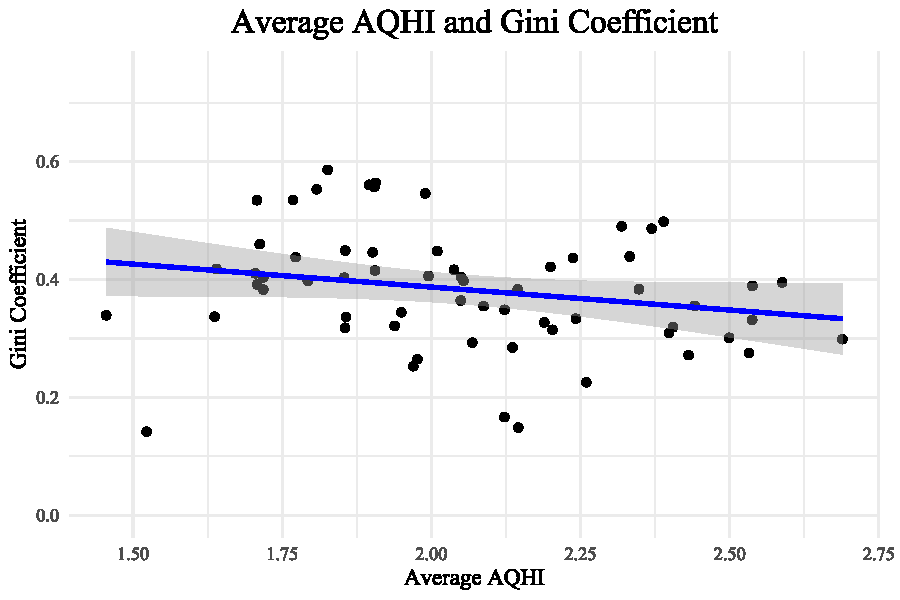
\includegraphics[width=0.8\textwidth]{aqhi_gini_plot.pdf}
\caption{Scatterplot and Bivariate Regression of CMA Average AQHI and Gini Coefficient}
\label{fig:gini_aqhi}
\begin{figurenotes}
Scatterplot represents CMA data values for Average AQHI and Gini Coefficient. The
blue line represents the simple bivariate regression of the form $\hat{Y} = \beta_0
+ \beta_1 X_i$ where $\hat{Y}$ represents predicted Gini Coefficient, $\beta_0$ 
represents the predicted intercept, $\beta_1$ represents the coefficient on Average
AQHI, and $X_i$ represents a compact space of Average AQHI values such that $X_i
\in [1.455, 2.689]$: the range of our collected values of Average AQHI. $\beta_0$ had an
estimated value of 0.543 with a standard error of 0.090. $\beta_1$ had an estimated value
of -0.078 with a standard error of 0.043.
\end{figurenotes}
\begin{figurenotes}[Source]
Environment and Climate Change Canada, 2025; Statistics Canada, 2021a;
Statistics Canada, 2021b; \\Environics Analytics, 2024.
\end{figurenotes}
\end{figure}

\section{Model Specification}

\subsection{Main Model Specification}

The core objective of this model is to estimate the effect of air quality (as 
captured by AQHI) on income inequality (as measured by the Gini Coefficient)
within CMAs. To investigate the relationship between air quality and income 
inequality, we employ an ordinary least squares (OLS) regression model with the
functional form:
\begin{equation}
Gini_i=\beta_0+\beta_1 AQHI_i+\beta_2 AQHI_i \times IncomeCat_i
+\sum_{k=1}^{6} \left( \beta_{k+2} W_{k,i} \right)
+ \epsilon_i
\end{equation}
The dependent variable in this model is $Gini_i$, our estimation of the Gini
Coefficient. The independent variable of interest is $AQHI_i$, which is the
average AQHI in a given CMA. This captures typical air quality conditions,
accounting for various types of pollutants (Government of Canada, 2021). This 
model will directly test whether
\emph{ceteris paribus} differences in air quality are associated with changes in
the Gini Coefficient. For example, if the estimated coefficient $\beta_1$ on 
$AQHI_i$ is significant and positive, that would indicate that worse air quality
is correlated with higher income inequality within a CMA. We also have included 
an interaction variable constructed from $AQHI_i \times IncomeCat_i$, which is a 
categorical variable representing the mean income for a given CMA. We include 
this variable because we expect air quality to effect income inequality 
differently in places with higher or lower average incomes due to the heterogenous
health impacts of air pollution (Deryugina et. al, 2021). Adding in this 
interaction variable will not introduce endogeneity: mean income was not used in
our calculation of the Gini Coefficient, and the interaction variable only 
accounts for changes in the effect of $AQHI_i$ on $Gini$ across different
levels of average CMA income. Since we are not including average income directly,
we have centered and categorized CMA mean incomes. This will make our interpretation of 
the model more clear and avoid any problems caused by potential non-linearity in
the interaction variable. The variable $IncomeCat$ takes on three values: $IncomeCat_{Low}$,
corresponding to CMAs with a mean income in the bottom 33\% of all studied CMAs;
$IncomeCat_{Mid}$, corresponding to CMAs with a mean income in the middle 33\% of all
studied CMAs; and $IncomeCat_{High}$, corresponding to CMAs with a mean income in the 
top 33\% of all studied CMAs.

We have chosen the following control variables:
\begin{enumerate}
  \item Percent Male Population (\%)
  \item Percent of Population $>$15 Years Old Married or Living With A 
  Common-Law Partner (\%)
  \item Percent Immigrant Population (\%)
  \item Percent of Population $>$15 Years Old in the Labour Force (\%)
  \item Employment Rate (\%)
  \item CMA Land Area (km$^2$)
\end{enumerate}

Percent male population is included as a control variable because there is higher male representation in industries
like manufacturing, which are correlated with both air pollution and income
inequality (Alexikova et al., 2016). 

Marital status is included as a control variable: in lower-income regions, dual-income households
often exhibit higher financial stability than single-income households (Downey et
al., 2017). 

Percent immigrant population is included as a control variable because
recent immigrants tend to concentrate in low-income, high-pollution areas
(American Lung Association, 2023). Additionally, increases in income inequality
in Canada have historically been associated with immigrant populations (Picot and Hou, 2019).

We include labor force participation rate and employment rate to account for variations
in economic prosperity across CMAs.

CMA land area is included as a control variable to address potential heterogeneity
between CMAs caused by geographic fixed effects.
Geographically larger CMAs 
might vary in both pollution levels and income inequality; standardizing air quality 
and income inequality by land area adjusts for this fixed effect.

We ultimately decided to
omit two control variables to account for high multicollinearity. 
The percentage of immigrants in total population
has an extremely high correlation with both the percent of population with visible 
minority status ($\rho = 0.971$) and the percent of population without knowledge
of English or French ($\rho = 0.835$). As such, both of these variables
were not included in our regression.

We recognize the potential of omitted variables in our model; however, through
the inclusion of these control variables, we assume Conditional Mean Independence
such that the error term $\epsilon$ is not correlated with our independent variable
of interest $AQHI$: $E[\epsilon | AQHI] = 0$.

The error term represents unobserved factors influencing local income inequality
that are not explicitly included in the model.

\subsection{Model Variations}

To ensure the validity of our results, we propose four alternative models.

We first add $AQHI_i^2$ to our regression to account for a possible nonlinear effect of air
quality on income inequality. Different levels of environmental exposure to poor
air quality might be associated with varying health and economic consequences: by 
including both a linear and a quadratic term, we can test whether the effects of
higher pollutant concentrations follow a simple linear pattern or exhibit
diminishing/increasing marginal effects (Banzhaf \& Walsh, 2008; Landrigan et. al, 2018).
This gives us the following alternative functional form:
\begin{equation}
Gini_i=\beta_0+\beta_1 AQHI_i+\beta_2 AQHI_i^2 + \beta_3 AQHI_i \times IncomeCat_i
+\sum_{k=1}^{6} \left( \beta_{k+3} W_{k,i} \right)
+ \epsilon_i
\end{equation}

Next, we replace the interaction variable $AQHI_i \times IncomeCat_i$ with the
quadratic term $AQHI_i^2$. This change tests whether AQHI’s effect on income inequality
actually varies in CMAs with higher or lower average incomes: it's possible that
a direct nonlinear effect of air quality on income inequality is obscured by
the interaction variable. This gives us an alternative functional form:
\begin{equation}
Gini_i=\beta_0+\beta_1 AQHI_i+\beta_2 AQHI_i^2
+\sum_{k=1}^{6} \left( \beta_{k+2} W_{k,i} \right)
+ \epsilon_i
\end{equation}

Next, we remove the control variable for CMA land area to verify
that our results are not unduly influenced by the inclusion of geographic fixed
effects and that we are not overfitting our regression.
This gives us the following alternative functional form:
\begin{equation}
Gini_i=\beta_0+\beta_1 AQHI_i+\beta_2 AQHI_i \times IncomeCat_i
+\sum_{k=1}^{5} \left( \beta_{k+2} W_{k,i} \right)
+ \epsilon_i
\end{equation}

Finally, we group our data by CMA Census Population Designation to capture potential
heterogeneity caused by population size: more populous CMAs may vary in both pollution
levels and income inequality. This gives us a regression model of the functional form:
\begin{equation}
Gini_i=\beta_0+\beta_1 AQHI_i+\beta_2 AQHI_i \times IncomeCat_i
+\sum_{k=1}^{7} \left( \beta_{k+2} W_{k,i} \right)
+ \epsilon_i
\end{equation}

\section{Table of Results}
Table~\ref{tab:reg_results} displays the results of our main functional form, given by Equation (1) and
four alternative functional forms, given by Equations (2-5). Significance values of each coefficient 
estimate are noted.
\begin{table}[!htbp] \centering 
  \caption{Main Functional Form and Alternative Specifications:\\Determinants of Income 
  Inequality in Canadian CMAs ($n = 63$).} 
  \label{tab:reg_results} 
\begin{adjustbox}{max width=\textwidth}
\begin{tabular}{@{\extracolsep{5pt}}lccccc} 
\\[-1.8ex]\hline 
\hline \\[-1.8ex] 
 & \multicolumn{5}{c}{\textit{Dependent Variable: Gini Coefficient}} \\ 
\cline{2-6} 
\\[-1.8ex] & Main & Alt. 1 & Alt. 2 & Alt. 3 & Alt. 4 \\ 
\\[-1.8ex] Variable & (1) & (2) & (3) & (4) & (5) \\ 
\hline \\[-1.8ex] 
Intercept & 2.807$^{***}$ & 3.424$^{***}$ & 3.591$^{***}$ & 2.766$^{***}$ & 2.791$^{***}$ \\
 & (0.319) & (0.459) & (0.701) & (0.343) & (0.325)  \\
\\
Average AQHI & 0.089$^{**}$ & $-$0.415 & $-$0.378 & 0.085$^{**}$ & 0.087$^{**}$ \\ 
 & (0.026) & (0.269) & (0.357) & (0.028) & (0.026)  \\ 
Average AQHI: Medium Income & $-$0.035$^{***}$ & $-$0.033$^{***}$ & --- & $-$0.032$^{***}$ 
& $-$0.036$^{***}$ \\ 
 & (0.008) & (0.008) &  & (0.008) & (0.009)  \\ 
Average AQHI: High Income & $-$0.064$^{***}$ & $-$0.065$^{***}$ & --- & $-$0.060$^{***}$ 
& $-$0.064$^{***}$ \\ 
 & (0.008) & (0.008) &  & (0.008) & (0.008) \\ 
(Average AQHI)$^2$ & --- & 0.123 & 0.093 & --- & ---  \\ 
 &  & (0.064) & (0.082) & & \\ 
\\
Male (\%) &  $-$0.046$^{***}$ & $-$0.047$^{***}$ & $-$0.036$^{**}$ & $-$0.042$^{***}$ 
& $-$0.046$^{***}$ \\ 
 & (0.007) & (0.007) & (0.012) & (0.008) & (0.008)  \\ 
Married (\%) & 0.003 & 0.002 & $-$0.001 & 0.003 & 0.003 \\ 
 & (0.003) & (0.003) & (0.003) & (0.003) & (0.003)  \\ 
Immigrant (\%) & $-$0.002$^{*}$ & $-$0.002$^{**}$ & $-$0.002$^{*}$ & $-$0.002$^{*}$ & $-$0.002$^{*}$ \\ 
 & (0.001) & (0.001) & (0.001) & (0.001) & (0.001)  \\ 
Employment Rate (\%) & $-$0.002 & $-$0.02 & $-$0.005 & $-$0.003 & $-$0.002  \\ 
 & (0.003) & (0.003) & (0.004) & (0.003) & (0.003)  \\ 
Labour Force (\%) & $-$0.004 & $-$0.004 & $-$0.010$^{***}$ & $-$0.004 & $-$0.004  \\ 
 & (0.002) & (0.002) & (0.003) & (0.002) & (0.003)  \\ 
Land Area (km$^2$) & $[+]$ & $[+]$ & $[-]$ & --- & $[+]$  \\ 
Grouped by Census Designation & --- & --- & --- & --- & \checkmark \\ 
\\ 
R$^{2}$ & 0.802 & 0.812 & 0.632 & 0.793 & 0.802 \\ 
Adjusted R$^{2}$ & 0.776 & 0.764 & 0.577 & 0.762 & 0.760 \\ 
\hline 
\hline \\[-1.8ex] 
\end{tabular} 
\end{adjustbox}
\\[1ex]
\begin{tablenotes}
Robust standard errors are listed in parentheses. Coefficient estimate significance
is indicated  as follows: $^{*}$: $p < 0.1$, $^{**}$: $p < 0.05$, $^{***}$: $p < 0.01$.
This table presents the results of OLS regressions estimating the relationship 
between Average AQHI and Gini Coefficient across Canadian Census Metropolitan Areas (CMAs). 
Average AQHI is the independent variable of interest in all models.
The main functional form, shown in Equation (1), includes an interaction variable 
between Average AQHI and CMA Mean Income.
Alternative specifications (2–5) test model robustness. Alt. 1 is the functional form
described in Equation (2) which adds (Average AQHI)$^2$. Alt. 2 is the functional form
described in Equation (3) which replaces the interaction variable between Average AQHI
and CMA Mean Income with (Average AQHI)$^2$. Alt. 3 is the functional form described
in Equation (4) which omits the Land Area control variable. Alt. 4 is the functional
form described in Equation (5) which groups CMAs by Census Designation. The coefficient estimate
$\beta_8$ for Land Area is non-significant with a magnitude $|\beta_8| < 10^{-5}$
in all functional forms; the sign of the coefficient estimate is noted.
\\
\end{tablenotes}
\begin{tablenotes}[Source]
Environment and Climate Change Canada, 2025; Statistics Canada, 2021a;
Statistics Canada, 2021b; \\Environics Analytics, 2024.
\end{tablenotes}
\end{table} 

\section{Discussion}
\subsection{Results}
\textbf{Our findings suggest that Average AQHI is a significant determinant of Gini Coefficient
in Canadian CMAs.} In our main functional form, the coefficient estimate $\beta_1$ on
Average AQHI is 0.089 ($p = 0.0013$). This coefficient estimate is statistically significant
and positive; holding all other factors constant, a 1-unit increase in Average AQHI in a
low-income CMA increases that CMA's expected Gini Coefficient by 0.089.

In all functional forms containing the interaction variable $AQHI_i \times IncomeCat_i$,
the coefficient estimates $\beta_{2a}$ and $\beta_{2b}$ are statistically significant.
In our main functional form, $\beta_{2a}$ has a coefficient estimate of -0.035
($p = 9.994 \times 10^{-5}$). Holding all other factors constant, in middle-income 
CMAs, a 1-unit increase in Average AQHI
increases a CMA's expected Gini Coefficient by 0.054. In our main functional form,
$\beta_{2b}$ has a coefficient estimate of -0.064 ($p = 3.437\times10^{-11}$). 
Holding all other factors constant, in high-income CMAs, a 1-unit increase in 
Average AQHI increases a CMA's expected Gini Coefficient by 0.026. 

Our main functional form has a high explanatory power (Adjusted R$^2$ = 0.776).
This confirms our hypothesis: there is a
significant, positive relationship between air pollution and income inequality. 
Additionally, the effect of Average AQHI on Gini Coefficient decreases in CMAs with a 
higher mean income: air pollution is associated with higher income inequality,
but air pollution has less of an impact on income inequality in wealthier CMAs.
These insights could help inform policy targeting environmental and social 
inequality. In particular, improving air quality in low-income CMAs could 
have a meaningful impact on reducing inequality.

All other variables included in the regression are control variables. We will 
not interpret the magnitude of their effect on estimated Gini Coefficient, but we should
evaluate the sign of their coefficient estimates for model robustness:
\begin{enumerate}
  \item $W_1$, Male (\%): $\beta_3 = [+]$, Expected (Alexikova et al., 2016)
  \item $W_2$, Married (\%): $\beta_4 = [+]$, Unexpected (Downey et al., 2017)
  \item $W_3$, Immigrant (\%): $\beta_5 = [-]$, Unexpected (American Lung Association, 2023; Picot and Hou, 2019)
  \item $W_4$, Employment Rate (\%): $\beta_6 = [-]$, Expected
  \item $W_5$, Labour Force (\%): $\beta_7 = [-]$, Expected
  \item $W_6$, Land Area (km$^2$): $\beta_8 = [+]$, Expected
\end{enumerate}

A positive coefficient estimate on $W_1$ is expected: there is higher male representation
in industries like manufacturing, which are associated with income inequality (Alexikova et. al, 2016).

A positive coefficient estimate on $W_2$ is unexpected: since dual-income households 
often exhibit higher financial stability than single-income households, one may expect
to see decreased income inequality in CMAs with a higher proportion of dual-income households
(Downey et al., 2014). However, the percentage of married or common-law partners in a 
CMA does not necessarily indicate the number of dual-income households in a CMA. It is possible
that a different unknown effect is present.

A negative coefficient estimate on $W_3$ is unexpected: 
increases in income inequality in Canada have historically 
been associated with immigrant populations (Picot and Hou, 2019). However, this may no longer
be the case. The proportion of immigrant populations in Canada have continually increased
since the 1950s, so it is possible that the relationship between immigrant population and 
income inequality has changed (Statistics Canada, 2016). CMAs with a high proportion of
immigrants may have significant immigrant communities who have developed effective
systems of community resilience.

A negative coefficient estimate on $W_4$ is expected: CMAs with a higher employment
rate are likely to have fewer households with no income, thereby decreasing income
inequality. Similarly, a negative coefficient estimate on $W_5$ is also expected:
CMAs with a high labour force integration can be expected to have fewer households
with no income, thereby decreasing income inequality. Finally, a positive coefficient
estimate on $W_6$ is expected: CMAs with higher land area may have increased variance
in income due to urban sprawl, differences in available opportunities between communities,
and higher industrialization.

\subsection{Validation Tests}

To assess whether our main functional form is correctly specified with low multicollinearity
and heteroskedasticity, we run a Ramsey RESET test, calculate Variance Inflation Factors (VIF), 
and run a White's test.

For the Ramsey RESET test, our null hypothesis $H_0$ is that an equation of
the functional form
\begin{equation}
Gini_i=\beta_0+\beta_1 AQHI_i+\beta_2 AQHI_i \times IncomeCat_i
+\sum_{k=1}^{6} \left( \beta_{k+2} W_{k,i} \right) 
+ \gamma_1 (\widehat{Gini_i})^2 + \gamma_2 (\widehat{Gini_i})^3
+ \epsilon_i \text{,}
\end{equation}
where $\widehat{Gini_i}$ is the predicted value of $Gini_i$ obtained from Equation (1),
has coefficient estimates $\gamma_1 = \gamma_2 = 0$. Our alternative hypothesis $H_1$ is that
at least one of $\gamma_1$, $\gamma_2 \neq 0$. Performing an F-test, we get $F=2.0131$
($p = 0.1441$) and fail to reject the null hypothesis: our functional form is not misspecified.

Since this functional form includes an interaction variable, the R function \verb|vif()| returns
generalized VIF values (GVIF). All calculated GVIF values are below 3. All GVIF values are 
presented in Table~\ref{tab:vif}.

\begin{table}[htbp]\centering
\caption{Main Functional Form: Generalized Variance Inflation Factors ($n = 63$)}
\label{tab:vif}
\begin{adjustbox}{max width=\textwidth}
\begin{tabular}{lrrrrrrrr}
\toprule
\textbf{Variable} & \textbf{A.A.} & \textbf{I.C.} & \textbf{M.P.} & 
\textbf{M.C.} & \textbf{I.} & \textbf{E.R.} &
\textbf{L.F.} & \textbf{L.A.}\\
\midrule
\textbf{GVIF} & 2.018 & 2.018 & 1.469 & 1.289 & 1.694 & 1.382 & 2.619 & 1.195 \\
\textbf{D.F.} & 3 & 3 & 1 & 1 & 1 & 1 & 1 & 1 \\
\bottomrule
\end{tabular}
\end{adjustbox}
\\[1ex]
\begin{tablenotes}
GVIF represents Generalized Variance Inflation Factors. D.F. represents degrees
of freedom. A.A. represents Average AQHI. I.C. represents Income Category. 
M.P. represents Male Population (\%). M.C. represents Married or Common-law (\%).  I. represents Immigrant (\%).
E.R. represents Employment Rate (\%). L.F. represents Labour Force (\%). L.A. represents Land Area (km$^2$).
\end{tablenotes}
\begin{tablenotes}[Source]
Environment and Climate Change Canada, 2025; Statistics Canada, 2021a;
Statistics Canada, 2021b; \\Environics Analytics, 2024.
\end{tablenotes}
\end{table}

Constructing our White's test, we have a null hypothesis $H_0$ that our error term is
homoskedastic such that $var \left(u_i | X_i = x \right) = c$, where $c \in \mathbb{R}$ is a constant.
Our alternate hypothesis $H_1$ is that our error term is heteroskedastic.
The result of our White's test, $\chi^2 = 0.12$ ($p=0.941$), does not indicate heteroskedasticity in our main functional form:
we fail to reject the null hypothesis.

\section{Specification Checks}

In our first alternate functional form described in Equation (2), we introduced the quadratic
term $AQHI^2_i$ to determine whether different levels of Average AQHI are
associated with different effects of Average AQHI on Gini Coefficient. From the
results of our regression detailed in Table~\ref{tab:reg_results}, it seems unlikely
that this is the case. Adding this quadratic term dramatically impacted the of the coefficient
estimate $\beta_1$ of $AQHI_I$: $\beta_1$ is now negative and nonsignificant (-0.415, $p=0.1283$).
The coefficient estimate $\beta_2$ of $AQHI^2_i$ is 0.123 ($p = 0.0602$). This suggests an initially negative,
concave upward relationship between $AQHI$ and $Gini$. However, because these results are not significant,
we cannot make inferences from this functional form. Additionally, the coefficient estimates
$\beta_{3a}$ and $\beta_{3b}$ of the interaction variable $AQHI_i \times IncomeCat_i$ were not dramatically
impacted by the inclusion of $AQHI^2_i$ (-0.033, $p = 0.0002$; -0.065, $p = 1.421\times 10^{-11}$). 
This functional form has less explanatory power than our main functional form (Adjusted R$^2$ = 0.764).


In our second alternate functional form described in Equation (3), we replaced the
interaction variable $AQHI_i\times IncomeCat_i$ with the quadratic term $AQHI^2_i$
to determine whether a direct nonlinear effect of air quality on income inequality
is obscured by the inclusion of the interaction variable. Once again, adding
this quadratic term dramatically impacted the of the coefficient
estimate $\beta_1$ of $AQHI_I$: $\beta_1$ is now negative and nonsignificant (-0.379, $p=0.2742$).
The coefficient estimate $\beta_2$ of $AQHI^2_i$ did not dramatically change (0.093, $p = 0.2579$).
Because these results are not significant, we cannot make inferences from this functional form.
The explanatory power of this functional form is considerably lower than our main functional form and
other specifications (Adjusted R$^2$ = 0.577). The interaction variable $AQHI_i \times IncomeCat_i$
seems to substantially contribute to the explanatory power and significance of our model.

In our third alternate functional form described in Equation (4), we removed our control
variable for CMA land area to verify that our results are not biased by the inclusion of
geographic fixed effects. Removing this variable did not dramatically impact the coefficient
estimate $\beta_1$ of $AQHI_I$ (0.085, $p=0.0043$) or the coefficient estimates
$\beta_{2a}$ and $\beta_{2b}$ of the interaction variable $AQHI_i \times IncomeCat_i$
(-0.031, $p = 0.0002$; -0.060, $p = 2.120\times 10^{-8}$). This functional form has
less explanatory power than our main functional form (Adjusted R$^2$ = 0.762). Removing this control
variable only negatively impacts our regression model: our main functional form is more effective.

In our fourth alternate functional form described in Equation (5), we grouped our data
by CMA Census Population Designation to capture potential heterogeneity caused by population size.
Adding this control variable did not dramatically impact the coefficient
estimate $\beta_1$ of $AQHI_I$ (0.087, $p=0.0017$) or the coefficient estimates
$\beta_{2a}$ and $\beta_{2b}$ of the interaction variable $AQHI_i \times IncomeCat_i$
(-0.036, $p = 0.0001$; -0.064, $p = 2.036\times 10^{-10}$). This functional form has
less explanatory power than our main functional form (Adjusted R$^2$ = 0.760). Adding this control
variable only negatively impacts our regression model: our main functional form is more effective.

\section{Robustness Analysis}

To further scrutinize the accuracy of our main regression model, we 
evaluate it through a quantile regression with $\tau=0.5$.

Quantile regression is less sensitive to outliers, thereby allowing us to see how coefficient
estimates differ at various percentiles of the conditional Gini Coefficient distribution. By 
focusing on the median of $Gini$ by using $\tau = 0.5$, we can evaluate whether the effect of $AQHI_i$
on $Gini$ remains accurate near the middle of the distribution. If the estimated coefficients on $AQHI_i$ 
and $AQHI_i \times IncomeCat_i$ remain significant and keep the same sign in the quantile regression
as calculated by Equation (1), this would affirm that the estimated relationship between
$AQHI_i$ and $Gini$ is not merely driven by outliers or skewed distributions in either 
extreme (e.g., extremely unequal or extremely equal CMAs).

\begin{table}[!htbp] \centering 
  \caption{Quantile Regression:\\Determinants of Income 
  Inequality in Canadian CMAs ($n = 63$).} 
  \label{tab:quantreg} 
\begin{adjustbox}{max width=\textwidth}
\begin{tabular}{@{\extracolsep{5pt}}lccc} 
\\[-1.8ex]\hline 
\hline \\[-1.8ex] 
 & \multicolumn{3}{c}{\textit{Dependent Variable: Gini Coefficient}} \\ 
\cline{2-4} 
\\[-1.8ex] Variable & Coefficient Estimate & Lower Bound & Upper Bound \\ 
\hline \\[-1.8ex] 
Intercept & 2.906 & 1.778 & 3.064 \\
\\
Average AQHI & 0.081 & 0.14 & 0.131\\
Average AQHI: Medium Income & $-$0.025 & $-$0.054 & $-$0.014 \\ 
Average AQHI: High Income & $-$0.056 & $-$0.069 & $-$0.038 \\
\\
Male (\%) & $-$0.046 & $-$0.052 & $-$0.030 \\ 
Married (\%) & 0.004 & 0.001 & 0.007 \\ 
Immigrant (\%) & $-$0.002 & $-$0.003 & $-$0.001 \\ 
Employment Rate (\%) & $-$0.004 & $-$0.008 & 0.001 \\ 
Labour Force (\%) & $-$0.002 & $-$0.008 & 0.001 \\ 
Land Area (km$^2$) & $[+]$ & $[+]$ & $[+]$ \\ 
\hline 
\hline \\[-1.8ex] 
\end{tabular} 
\end{adjustbox}
\\[1ex]
\begin{tablenotes}
This table shows the results of a quantile regression using the functional form
described in Equation (1) and $\tau = 0.5$.
Lower Bound and Upper Bound refer to a 95\% confidence interval constructed
around the coefficient estimate.
\\
\end{tablenotes}
\begin{tablenotes}[Source]
Environment and Climate Change Canada, 2025; Statistics Canada, 2021a;
Statistics Canada, 2021b; \\Environics Analytics, 2024.
\end{tablenotes}
\end{table} 

While the coefficient estimate of $\beta_1$ on $AQHI_i$ shifts modestly ($-$0.008), its 
sign remains positive. Additionally, the 95\% confidence interval constructed around
the coefficient estimate of $\beta_1$ does not include $\beta_1 = 0$, suggesting 
that this coefficient estimate remains significant. Additionally, the coefficient estimates
of $\beta_{2a}$ and $\beta_{2b}$ on $AQHI_i \times IncomeCat_i$ have retained their
sign and are significant.

This robustness check suggests that the relationship between 
$AQHI_i$ and $Gini$ is not merely driven by outliers or skewed distributions.
Our main model, described in Equation (1), remains an effective estimation of the
relationship between $AQHI_i$ and $Gini$.

\section{Conclusion}

This study finds a significant, positive relationship between Average 
AQHI and Gini Coefficient within Canadian CMAs ($\beta_1 = 0.089$, $p = 0.0013$). 
Additionally, the effect of Average AQHI 
on Gini Coefficient decreases in CMAs with a higher mean income ($\beta_{2a} = -0.035$,
$p = 9.994 \times 10^{-5}$; $\beta_{2b} = -0.064$, $p = 3.437\times10^{-11}$). 
\textbf{This suggests that air pollution is associated with higher income inequality in Canadian
Census Metropolitan Areas, and that air pollution has a weakened effect on income inequality 
in wealthier Census Metropolitan Areas.} 

These findings suggest that there is a possible destabilizing effect of air pollution 
on income equality. This brings into question the conclusions argued by Jha et al. (2019).
Stringent air quality regulations may only be associated with heightened income inequality
because air pollution worsens or prolongs the effect of an economic shock on income inequality.
The findings of this paper demand further research: future works should seek to identify
the relationship between air pollution and an economy’s resilience to income inequality.
Future studies could employ panel data to evaluate this relationship, establish causality, and identify 
the mechanisms through which poor air quality contributes to heightened inequality.

Additionally, these findings indicate that air quality regulation may improve—rather
than exacerbate—income inequality. Additional environmental intervention in Canadian 
Census Metropolitan Areas with high Average AQHI readings could help mitigate income inequality. 

\section{References}



References here (manual or bibTeX). If you are using bibTeX, add your bib file 
name in place of BibFile in the bibliography command.
% Remove or comment out the next two lines if you are not using bibtex.
\bibliographystyle{aea}
\bibliography{BibFile}

% The appendix command is issued once, prior to all appendices, if any.
\appendix

\section{A: Mathematical Analysis}

$\beta_1$

\end{document}

